\documentclass[conference]{IEEEtran}
\usepackage[hidelinks=true]{hyperref}
\usepackage{cite}
\usepackage{amsmath,amssymb,amsfonts}
\usepackage{algorithmic}
\usepackage[brazil]{babel}
\usepackage[utf8]{inputenc}
\usepackage{graphicx}
\usepackage{textcomp}
\usepackage{xcolor}
\hypersetup{frenchlinks=true}
%\hypersetup{colorlinks=false,pdfborder={0 0 0}}

\def\BibTeX{{\rm B\kern-.05em{\sc i\kern-.025em b}\kern-.08em
    T\kern-.1667em\lower.7ex\hbox{E}\kern-.125emX}}
\begin{document}

\title{Trabalho de Programação}
%----------------------------------------------------------------------------------------------------------
\author{\IEEEauthorblockN{Pablo Freitas Santos}

\IEEEauthorblockA{\textit{Engenharia Mecatrônica} \\
\textit{Universidade Federal de Santa Catarina}\\
Joinville, Brasil \\
pablo.freitas@grad.ufsc.br}
}
%----------------------------------------------------------------------------------------------------------
\maketitle
%----------------------------------------------------------------------------------------------------------
\begin{abstract}

Esse trabalho tem objetivo de implementar um algoritmo de uma fila em que representa a pista de pouso e decolagem de um aeroporto e trabalhando o conceito de classes e construir um diagrama do algoritmo.


\end{abstract}

\begin{IEEEkeywords}
classe, fila, diagrama
\end{IEEEkeywords}
%---------------------------------------------------------------------
\section{Introdução}
Para a construção da classe \texttt{Extended\_queue} inicialmente pensou-se na organização de memória separada para cada função e em seguida como liberar para evitar vazamentos. Depois um diagrama de classes de acordo com o UML e com o objetivo de separar a acessibilidade e os tipos de relacionamentos que cada classe possui.
 
%--------------------------------------------------------------
\section{Desenvolvimento}
%comentários breves sobre a implementação no desenvolvimento.

A partir da inclusão das bibliotecas foi feito o construtor da \texttt{Extended\_queue}, que basicamente inicializava a fila da forma padrão, primeiro e último nó nulos e tamanho igual a zero. Em seguida no destrutor foi chamada a função \texttt{Extended\_queue::serve()} enquanto a fila não estivesse vazia, evitando-se assim vazamentos de memória.

%Para que não houvesse quebra do privado e público foram dadas funções ditas como básicas para ter acesso ao privado sem quebrar o conceito de acessibilidade. Como por exemplo, \texttt{Extended\_queue::getFirstNode()}, que faz parte da \texttt{class Extended\_queue}, que foi implementada exclusivamente para ter acesso a informações que estão no privado.

A maiorias das funções não houve problemas de implementação, no entanto \texttt{Error\_code Extended\_queue::append(Plane \&plane)} teve a necessidade de pensar nos modos que poderiam corromper o algoritmo para se adequar aos retornos e \texttt{Error\_code} e avaliar os casos de colocar em uma fila vazia ou colocar em uma fila que já possui elementos.

Na construção do diagrama(\autoref{b2}) foi utilizado a ferramenta Umbrello\cite{b4}, e no caso desse algoritmo só foi encontrado 2 tipos de associações entre classes, agregação simples(losango vazado), demonstra que as informações de um objeto precisam ser complementadas por um objeto de outra classe (objeto - todo) e composição (losango preenchido), que representa um vínculo mais forte entre objetos-todo e objetos-parte. Objetos-parte têm que pertencer ao objeto-todo\cite{b5}.
%\begin{figure}[htb]
%	\caption{\label{Complete}Completo}
	%\begin{center}
	%    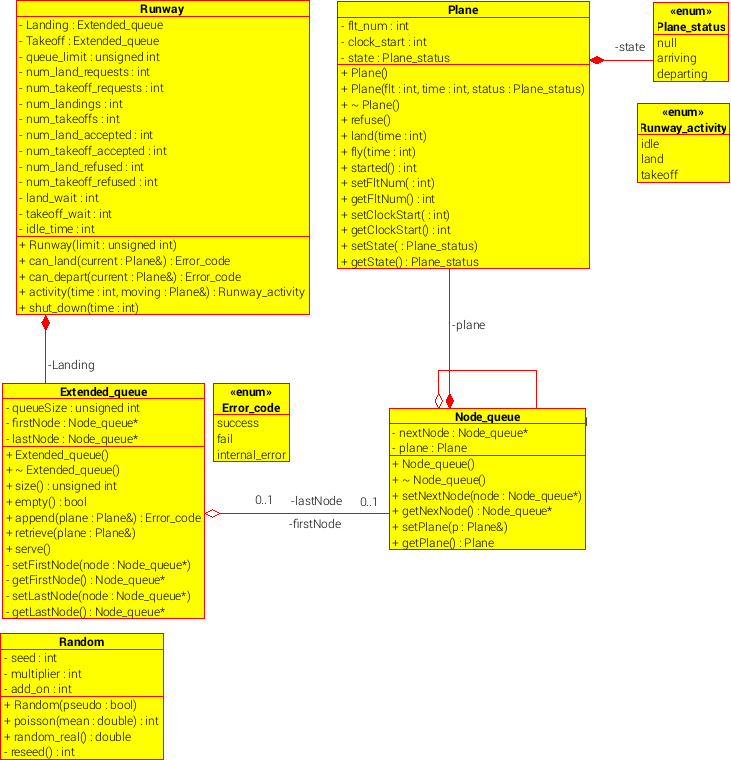
\includegraphics[scale=0.6]{figs/airport_.png}
	%\end{center}
	%\legend{Fonte:Elaborado pelo autor}
%\end{figure}

\begin{figure}[htb]
	\caption{\label{b2}Diagrama de classes do aeroporto}
	\begin{center}
	    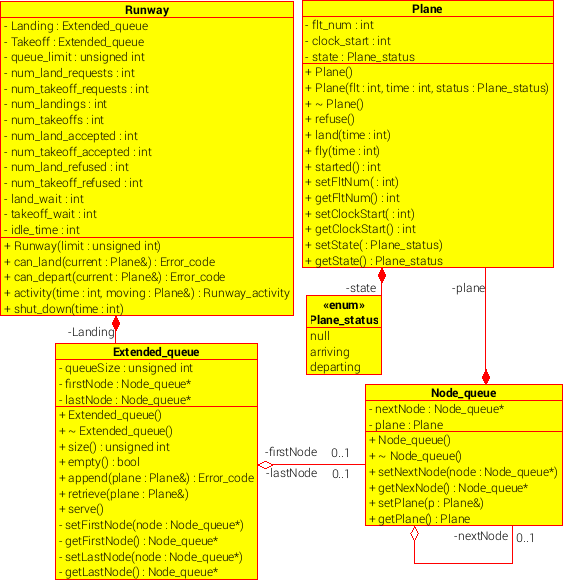
\includegraphics[scale=0.6]{figs/Parte_1.png}
	\end{center}
	%\legend{Fonte:Elaborado pelo autor}
\end{figure}

\begin{figure}[htb]
	\caption{\label{b3}Classes independentes}
	\begin{center}
	    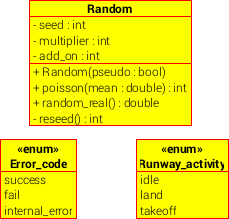
\includegraphics[scale=0.6]{figs/independt.png}
	\end{center}
	%\legend{Fonte:Elaborado pelo autor}
\end{figure}

\section{Conclusão}

Nesse projeto pode ser observado que cada classe possui uma importância para o algoritmo e devemos levar em conta a relação com as outras classes para construir diagramas que representando a acessibilidade de cada classe e separar cada classe por função.




\begin{thebibliography}{00}

\bibitem{b1} {Paul Deitel and Harvey Deitel. 2013. C++ how to Program (Early Objects Version) Deitel (9th ed.). Prentice Hall Press, Upper Saddle River, NJ, USA. 
}
\bibitem{b4}{\url{https://umbrello.kde.org/}}

\bibitem{b5}\url{http://homepages.dcc.ufmg.br/~figueiredo/disciplinas/aulas/uml-diagrama-classes-relacionamentos_v01.pdf}
\end{thebibliography}

%\begin{anexosenv}
%\partanexos

%\end{anexosenv}


\end{document}
